\chapter{The Genesis of a new asbtraction layers: Views}

\chapter{Upgrading the way to design IP algorithms}

\section{Keeping properties}

\section{Lazy evaluation}

\section{Composability and piping}

\chapter{A practical example: border management}

\chapter{Performance discussion}


\chapter*{Material about views}

\section{Introducing range-based image traversing}
\label{sec.range.traversing}

Previously in Milena~\cite{levillain.2009.ismm} we had a very customized way of traversing images: macro-based. It aimed
at hiding the complexity of such a task while loosing as little performance as possible. For example, the dilation
algorithm was written this way:

\begin{minted}{c++}
  template<class I, class SE>
  mln_concrete(I) dilate(const I& f, const SE& se)
  {
    mln_concrete(I) g;
    initialize(g, f);
    mln_piter(I) p(f.domain());
    mln_qiter(SE) q(se, p);
    for_all(p) // for all p in f domain
    {
      mln_value(I) v = f(p);
      for_all(q) // for all q in se(p)
        if(f.has(q) and f(q) > v)
          v = f(q);
      g(p) = v;
    }
    return g;
  }
\end{minted}

In this code \texttt{mln\_concrete}, \texttt{mln\_piter}, \texttt{mln\_qiter}, \texttt{for\_all} and \texttt{mln\_value}
are all macros aiming at hiding the underlying complexity. Our goal is to replace those macros with existing C++ core
language code to improve the user experience as well as ease the maintenance, contribution and further improvement of
the library. Nowadays, a tool named range (and especially Eric Niebler's range-v3) allow seamless traversing of an
image. For instance, we can rewrite the above algorithm this way:

\begin{minted}{c++}
  template<class I, class SE>
  image_concrete_t<I> dilate(const I& f, const SE& se)
  {
    auto g = f.concretize();
    auto supr = accu::supremum<image_value_t<I>>();
    for(auto [f_px, g_px] : zip(f.pixels(), g.pixels()))
    {
      for(auto qx : se(f_px))
        supr.take(qx.val());
      g_px.val() = supr.result();
    }
    return g;
  }
\end{minted}

Here we have a much more efficient code that, in theory, enables compiler optimizations such as vectorization or inner
loops unrolling. But through benchmarking, we have learned that this solution doesn't mix well with the multidimensional
nature of images. The issue originates from the fact that we have no way to explicitly say in the code that the
multidimensional range is made of chunk of contiguous rows of memory. Indeed, for each element we have to compute an
index originating from potentially $N$ dimensions. This disables critical optimizations such as vectorization.

We solved this problem by augmenting range-v3's ranges with our own multidimensional ranges. Indeed, we only need to
have contiguity on the last dimension to provide the compiler code it can optimize. Which means that each for-loop that
traverses the whole n-dimensional image can be transformed into a double for-loop whose inner loop is guaranteed to be a
contiguous row. This way we have now an outer range as well as an inner range, as illustrated in
figure~\ref{fig.inner.outer.range}.

\begin{figure}[htbp]
  \centering
  \subcaptionbox{}{\includegraphics[width=.48\linewidth]{svg-inkscape/linear_rng_svg-tex.pdf}}
  \subcaptionbox{}{\includegraphics[width=.48\linewidth]{svg-inkscape/segmented_rng_svg-tex.pdf}}
  \caption{Range-v3's ranges (a) vs. multidimensional ranges (b).}
  \label{fig.inner.outer.range}
\end{figure}

Thanks to this new design we can now rewrite our algorithm with a double for-loop for the image traversing. Hopefully it
stays really similar to what one would be used to when working with the classical two dimension image. As an example, we
can rewrite the dilation algorithm this way:

\begin{minted}{c++}
  template<class I, class SE>
  image_concrete_t<I> dilate(const I& f, const SE& se)
  {
    auto g = f.concretize();
    auto supr = accu::supremum<image_value_t<I>>();
    auto zipped_pixels = zip(f.pixels(), g.pixels());
    for(auto&& row : ranges::rows(zipped_pixels))
      for(auto [f_px, g_px] : row)
      {
        for(auto qx : se(f_px))
          supr.take(qx.val());
        g_px.val() = supr.result();
      }
    return g;
  }
\end{minted}

The highlight of this code is the usage a new tool: \texttt{ranges::rows} to bring out an inner range (contiguous) from
the multidimensional outer range.


\section{Introducing Views}
\label{sec.views}

\subsection{Practical genericity for efficiency: the Views}
\label{subsec.views}

Let us introduce another key point enabled by genericity and concepts: the \emph{Views}. A \emph{View} is defined by a
non-owning lightweight image, inspired by the design introduced in \emph{Ranges for the Standard
  Library}~\citep{niebler.2014.ranges} proposal for \emph{non-owning collections}. A similar design is also called
\emph{Morphers} in \textsc{Milena}~\citep{levillain.2009.ismm, geraud.2012.hdr}. \emph{Views} feature the following
properties: \emph{cheap to copy}, \emph{non-owner} (does not \emph{own} any data buffer), \emph{lazy evaluation}
(accessing the value of a pixel may require computations) and \emph{composition}. When chained, the compiler builds a
\emph{tree of expressions} (or \emph{expression template} as used in many scientific computing libraries such as
Eigen~\cite{guennebaud.2010.eigen}), thus it knows at compile-time the type of the composition and ensures a 0-overhead
at evaluation.

There are four fundamental kind of views, inspired by functional programming paradigm: \texttt{transform(input, f)}
applies the transformation $f$ on each pixel of the image \emph{input}, \texttt{filter(input, pred)} keeps the pixels of
\emph{input} that satisfy the predicate \emph{pred}, \texttt{subimage(input, domain)} keeps the pixels of \emph{input}
that are in the domain \emph{domain}, \texttt{zip($input_1$, $input_2$, \ldots, $input_n$)} allows to pack several pixel
of several image to iterate on them all at the same time.

\emph{Lazy-evaluation} combined with the view \emph{chaining} allows the user to write clear and very efficient code
whose evaluation is delayed till very last moment as shown in~\cref{fig.lazy} (see \cite{geraud.2018.gtgdmm} for
additional examples). Neither memory allocation nor computation are performed; the image $i$ has just recorded all the
operations required to compute its values.

\begin{figure}[htbp]
  \begin{minipage}[l]{0.48\linewidth}
    \begin{minted}{C++}
image2d<rgb8>  ima1 = /* ... */;
image2d<uint8_t> ima2 = /* ... */;

// Projection: project the red channel value
auto f = view::transform(ima, [](auto v) {
  return v.r;
});

// Lazy-evaluation of the element-wise
// minimum
auto g = view::transform(view::zip(f, ima2),
  [](auto value) {
    return std::min(std::get<0>(value),
             std::get<1>(value));
});
\end{minted}
  \end{minipage}
  \hfill
  \begin{minipage}[l]{0.48\linewidth}
    \begin{minted}{C++}
// Lazy-Filtering: keep pixels whose value
// is below < 128
auto h = view::filter(g, [] (auto value) {
  return value < 128;
}));

// Lazy-evaluation of a gamma correction
using value_t = typename Image::value_type;
constexpr float gamma = 2.2f;
constexpr auto max_val =
  std::numeric_limits<value_t>::max();
auto i = view::transform(h,
  [gamma_corr = 1 / gamma] (auto value) {
    return std::pow(value / max_val,
             gamma_corr) * max_val;
});
\end{minted}
  \end{minipage}

  \caption{Lazy-evaluation and \emph{view} chaining.}
  \label{fig.lazy}
\end{figure}

\noindent The tree of type resulting from this view chaining is illustrated by~\cref{fig.viewAST}.

\begin{figure}[htb]
  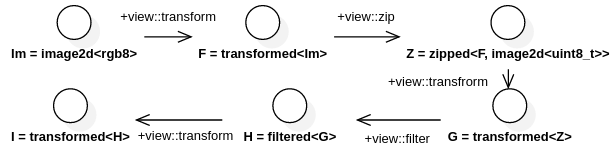
\includegraphics[height=2cm]{figs/viewAST.png}
  \caption{Abstract Syntax Tree of the types chained by the code above}
  \label{fig.viewAST}
\end{figure}

The concept of \emph{View} brought to us a fundamental issue when dealing with images: \blockquote{\emph{What is an
    image?}}. More precisely: should an image always be the owner of its data buffer? Should we have a shared ownership of
the data buffer between all the images using it? Then what happens when the data changes? The issue about the semantic
of an image is crucial but also very similar to the issue there is to differentiate a \emph{container} (such as
\texttt{std::vector}, that is to say the data buffer) and a \emph{view} on this container in the \emph{Ranges TS}.

From here we have considered two approaches. The first one is to have \emph{shared ownership} of the data buffer for the
image and its derived views. However this does not allow the differentiation between an already computed image and a
lazy image. To be able to make this differentiation is crucial in an \emph{Image Processing library} as we want to make
the most out of the data we already have and we do not want to compute data we do not need. Also, we cannot distinguish
when the \emph{copyability} property is required. This is the main reason why we did not adopt this approach.

The second one is to make the differentiation between a \emph{concrete image} which owns the data (like the standard
containers) and the \emph{views} that are lightweight cheap-to-copy objects. Not all \emph{concrete image} may be
\emph{copyable}, but all \emph{views} are. This is a very important property as it simplify greatly the reasoning when
performance is needed. It also enables us to have a library design similar to the standard library which the user is
familiar with and, why not, have standard algorithm and standard view work on our images types. All of these are the
main reason why we decided to adopt this design. Henceforth from now on the \emph{Image} concept is similar to the
\emph{View} concept from which we refines a \emph{ConcreteImage} concept that requires a specific behavior as it owns
data.


\vspace{1cm}

In~\cref{subsec.gen.concept}, we saw that what is truly important is the behavior: an algorithm will require its input
to be able to behave a certain way, and if those requirements are fulfilled, then the algorithm can be used with this
set of inputs. This enables non-standard type of image to be input in algorithms, providing they still behave correctly.
The way how we can check if the required behavior is satisfied is a new C++20 feature called \emph{concept} (the authors
show how to leverage them in~\cite{roynard.2019.rrpr}) that will not be presented in this paper. Additionally to
concepts, C++20 introduces a new library facility called \emph{ranges}~\cite{niebler.2018.deepranges} which includes a
non-owning lightweight container called \emph{views} whose design is very similar to that of \emph{morphers}, introduced
in Milena~\cite{levillain.2009.ismm,geraud.2012.hdr}. Views are completely transferable to the image processing world.
Also, views feature interesting properties that an image processing practitioner will find to his taste.

A view is a \emph{lightweight object} that behaves exactly the same as an image: let $V$ be a view of an image defined
on $\mathcal{D}$ then we have $\forall{p}\in\mathcal{D}, v = V(p)$. It can be a random generator that yields a random
number each time $V(p)$ is called; a proxy to the underlying image that records the number of times each pixel is
accessed in order, for instance, to compare algorithm performance; a projection to a specific color channel; applying an
automatic gamma correction; restricting the definition domain $\mathcal{D}$; and so on.

A view is a \emph{non-owning}, \emph{cheap-to-copy} lightweight object that basically only \emph{records an operation}
and stores a pointer to an image. For instance, let us consider the view transform defined as follow $v = transform(u_1,
  u_2, \cdots, u_n, f)$ where $u_i$ are input images and $h$ a n-ary function. $transform$ returns an image generated from
the other image(s) as show in~\cref{fig.view.threshold}. Also, we can see that the view itself does not own any image
but just stores pointers as well as the operation ($h$). This means that, for instance, modifying the original values of
the image(s) will impact the values yield by the view. Finally, as the view is cheap-to-copy, it features a pointer
semantic that help the practitioner passing around his images by copy to his algorithms without worrying about heavy
buffer copies in the background.

\begin{figure}[tbh]
  \centering
  \begin{minipage}{\linewidth}
    \includestandalone[mode=image, width=.9\linewidth]{figs/transform_thresholding}
  \end{minipage}
  \caption{An image view performing a thresholding.}
  \label{fig.view.threshold}
\end{figure}

Another key point of views is the lazy evaluation. When an image is piped through a view, no computation is done. The
computation happens when the practitioner requests a value by doing $val = V(p)$. The implications are multiples: an
image can be piped into several computation-heavy views, some of which can be discarded later on, it won't impact the
performance. Also, when processing large images, applying a transformation on a part of the image is as simple as
restricting the domain with a view and applying the transformation to this resulting sub-image.

Views will also try to preserve properties of the original image when they can. That means that views can preserve the
ability of the practitioner to, for instance, write into this image. This may be a trivial property to preserve when
considering a view that restrict a domain, but when considering a view that transforms the resulting values, it is not.
Let us consider the projection $h: (r,g,b) \mapsto g$ that selects the green component of an RGB triplet. When piping
the resulting view into, for instance, a blurring algorithm, the computation will take place in place thanks to still
having the ability to write into the image. A legacy way of obtaining the same result would have been to create a
temporary single-channel image consisting of the green channel of the original RGB image so that the temporary image
could then be blurred. Then one would have needed to copy the values of the temporary image back into the green channel
of the original image. The comparison between the legacy way and the in-place way of doing this computation is shown
in~\cref{fig.legacy.vs.view}.

\begin{figure}[tbh]
  \centering
  \subfloat[Legacy pipeline with copy]{
    \includegraphics[width=1.6in,align=t]{figs/blur_copy}
  }
  \hfil
  \subfloat[Modern pipeline with view]{
    \includegraphics[width=1.6in,align=t]{figs/blur_inplace}
  }

  \caption{Comparison of a legacy and a modern pipeline using \colorbox{lightgreen}{algorithms} and
    \colorbox{thistle}{views}.}
  \label{fig.legacy.vs.view}
\end{figure}

On the other hand, when considering the view $g: (r,g,b) \mapsto 0.2126*r+0.7152*g+0.0722*b$ that compute the gray level
of a color triplet (as shown in~\cref{fig.view.grayscale}), the ability to write a value into the image is not
preserved. One would need an inverse function that is able to deduce the original color triplet from the gray level to
be able to write back into the original image.

\begin{figure}[tbh]
  \centering
  \includegraphics[width=.98\linewidth]{figs/views/transform_grayscale}
  \caption{Usage of transform view: grayscale.}
  \label{fig.view.grayscale}
\end{figure}

\begin{figure}[tbh]
  \includestandalone[mode=image, scale=0.6]{figs/clip}

  \includestandalone[mode=image, scale=0.6]{figs/filter}
  \caption{Clip and filter image adaptors that restrict the image domain by a non-regular ROI and by a predicate that
    selects only even pixels.}
  \label{fig.view.clip}
\end{figure}

Following the same principle, a view can apply a restriction on an image domain. In~\cref{fig.view.clip}, we show the
adaptor \texttt{clip(input, roi)} that restricts the image to a non-regular \texttt{roi} and \texttt{filter(input,
  predicate)} that restricts the domain based on a predicate. All subsequent operations on those images will only affect
the selected pixels.

\begin{figure}[tbh]
  \includestandalone[mode=image, scale=0.6]{figs/pipeline}
  \caption{Example of a simple image processing pipeline.}
  \label{fig.view.pipeline}
\end{figure}

Views feature many interesting properties that change the way we program an image processing application. To illustrate
those features, let us consider the following image processing pipeline: (Start) Load an input RGB-8 2D image (a
classical HDR photography) (A) Convert it in grayscale (B) Sub-quantize to 8-bits (C) Perform the grayscale dilation of
the image (End) Save the resulting 2D 8-bit grayscale image; as described in~\cref{fig.view.pipeline}.


\begin{figure}[tbh]
  \begin{minipage}{\linewidth}
    \includestandalone[mode=image, scale=0.59]{figs/composition}
  \end{minipage}
  \caption{Algorithm vs image view composition.}
  \label{fig.view.comp}
\end{figure}

\textbf{Views are composable.} Chaining operations has always been a very important feature in image processing as well
as in software engineering in general (known object composition). Being able to weave simple blocks together into more
complex blocks in a way that the resulting block can still be treated as a simple block is a most wanted feature.
The~\cref{fig.view.pipeline} features an example of a pipeline using 3 basic operations \emph{Image} $\rightarrow$
\emph{Image}: a grayscale conversion, a sub-quantization and a dilation. It is important to note that we can consider
there is only one complex operation composed of 3 basic algorithms in which an image is piped. A view thus carries both
information about the image and the transformations. In~\cref{fig.view.comp} we show the distinction between the
composition of algorithms and the compositions of views which carry both the image and the transformations.

\textbf{Views improve usability.} The code featuring the pipeline in~\cref{fig.view.comp} can almost be implemented the
following way:
\begin{minted}{c++}
auto input = imread(...);
auto A = transform(input, [](rgb16 x) -> float {
    return (x.r + x.g + x.b) / 3.f; };
auto MyComplexImage = transform(A, [](float x)
    -> uint8_t { return (x / 256 + .5f); };
\end{minted}
When one is familiar to functional programming, it is quite easy to draw the parallel between \emph{transform},
\emph{map}, \emph{filter} and the sequence operators. Views are, in reality, higher-order functions built from an image
as well as the function(s) (operator or predicate) to apply for each pixel. It is not required to make the iteration
over each pixel of the image oneself, we just provide the function to morph the image into another one. The technique
used when composition several sequence operators is called \emph{currying}~\cite{hanus.1995.curry} in the functional
programming world.

\textbf{Views improve re-usability.} When looking at the code snippets above, one could see that they are simple though
not very re-usable. However, keeping the functional programming paradigm in mind, one can easily define new views just
by considering that a view is a \emph{higher-order function}. Then, as shown in~\cref{fig.view.highorder}, the primitive
\emph{transform} serves as the basis to build three new views: one that performs the summation of two images, one that
performs the grayscale conversion and one that performs the sub-quantization. All those three views can then be reused
afterwards\footnote{A more generic implementation could have been provided for these views for even more re-usability,
  but this is not the purpose here.}.

\begin{figure}
  \noindent
  \begin{minted}{c++}
auto operator+(Image A, Image B) {
  return transform(A, B, std::plus<>());
}
auto togray = [](Image A) { return transform(A, [](auto x)
  { return (x.r + x.g + x.b) / 3.f; };)
};
auto subquantize16to8b = [](Image A) { return transform(A,
  [](float x) { return uint8_t(x / 256 +.5f); });
};

auto input = imread(...);
auto MyComplexImage = subquantize16to8b(togray(A));
  \end{minted}

  \caption{Using high-order primitive views to create custom view operators.}
  \label{fig.view.highorder}
\end{figure}

\textbf{Views for lazy computing.} One fundamental point of views is that they embed the operation within themselves,
meaning that in~\cref{fig.view.highorder}, the creation of the views does not incur any computation. The computation is
delayed until the invocation of the \texttt{v(p)} expression. Also, the computation can be delayed quite far thanks to
the composition capability of views. In fact, a view is an image adaptor which actually is a \emph{template
  expression}~\citep{veldhuizen.1995.expression, veldhuizen.2000.blitz}. Indeed, the \emph{expression} used to generate
the image is recorded as a template parameter. A view is represented by an \emph{expression tree}, as shown
in~\cref{fig.view.ast}.


\begin{figure}
  \null\hfill
  \begin{minipage}[b]{2cm}
    \includestandalone[mode=image, scale=0.8]{figs/view_ast}
  \end{minipage}
  \begin{minipage}[b]{5.5cm}
    \begin{minted}{c++}
Image f = ...; // grayscale
Image g = ...; // rgb16
Image out = subquantize16to8b(
              togray(g)) + f;
\end{minted}
  \end{minipage}
  \caption{View composition seen as an expression tree.}
  \label{fig.view.ast}
\end{figure}



\PLAGIAT{
  \textbf{Views for performance.} Consider a classical design where each operation of the pipeline is implemented on
  ``its own''. Each operation requires that memory be allocated for the output image, and also, each operation requires
  that the image be traversed. This design is simple, flexible, composable, but is not memory efficient nor
  computationally efficient. With the lazy evaluation approach, the image is traversed only once (when the dilation is
  applied) that has two benefits. First, there are no intermediate images so this is memory effective. Second, it is
  faster thanks to a better memory cache usage; processing a RGB16 pixel from the dilation algorithm directly converts
  it in grayscale, then sub-quantized it to 8-bits, and finally make it available. It acts \emph{as if} we were writing
  an optimal operator that would combine these operations.
}

\PLAGIAT{
  As an experiment, we benchmarked both pipelines on a 20MPix image RGB16 (random generated values) on a desktop
  computer i7-2600 CPU @ 3.40GHz, single-threaded\footnote{Experimentation code is available at
    \url{https://gitlab.lrde.epita.fr/mroynard/roynard.icip.2020.snippets}}. The dilation is done with a small 3x3 square
  structuring element using tiling for caching input values. The pipeline using views is about 20\% faster than the
  regular one (133 vs 106 ms). Note that views are also compatible with optimizations such as parallelization and
  vectorization.
}

\PLAGIAT{
  Background Subtraction: The background subtraction pipeline is used to detect changes in image
  sequences~\cite{opencv.bg_sub}. It is mainly used when regions of interest are foreground objects. The pipeline
  components include: subtraction, Gaussian filtering, threshold, erode and dilate, as shown
  in~\cref{fig.view.comp.sub_bg}.
}

\begin{figure}[tbh]
  \begin{minipage}{\linewidth}
    \includestandalone[mode=image, scale=0.59]{figs/pipeline_bg_sub_comp}
  \end{minipage}
  \caption{Background substraction pipeline using \colorbox{lightgreen}{algorithms} and
    \colorbox{thistle}{views}.}
  \label{fig.view.comp.sub_bg}
\end{figure}


\section{From local algorithm to border management}
\label{sec.localgo.bm}

In image processing there are three main families of algorithms:
\begin{itemize}
  \item Point-wise algorithms: they process each value of the image, individually from each others (e.g.
        multiplication).
  \item Local algorithms: they process each value of the image, helped with the knowledge of the neighboring values
        catched in a window: the structuring element (e.g. convolution).
  \item Global algorithms: they propagate the changes downstream during the algorithm unrolling. Knowledge of previously
        computed values is required (e.g. chamfer distance transform).
\end{itemize}
Here we are interested in particular in local algorithms. The long recurring issue is about the behavior on the border
of the image. There are many ways of dealing with this problem. One is to allocate additional memory for the border and
paste values in it. Another is to check the bounds when looping over the neighbors. We can also decorate the image to
return a correct lazily computed value when accessing out-of-image's-bound value still inside the extension. The point
is: all these methods have advantages as well as disadvantages.

\subsubsection{Memory allocated border}
The border width is fixed at the image's creation and cannot be augmented without doing a reallocation. There is also a
cost when computing border's values (to fill it) which is proportional to the border's width and to the image's size. On
the other hand, the access time of a border value during the algorithm unrolling is as fast as a native access time
within the image itself. The last issue remaining would be that the border is not infinite. We cannot process a local
algorithm with a structuring element that does not fit in the extension. This method is especially adapted when there is
medium structuring elements with a known size which will yield a lot of out-of-image's bound accesses. When speed is
required, this method is a defacto standard.

\subsubsection{Bound checking}
Assuming there is no border and we are not allowed to access out-of-image's-bound values, a bound check is required when
accessing each values. Another way to do would be to decorate the facility that yields the neighbors of a pixel: do not
yield out-of-image's-bound pixels. This removes the need to bound check for each pixel's value which is relatively
faster. The caveats of this method are that it induces a slight slow down when yielding the pixel's neighbors from the
structuring element, and that it is not always viable: some algorithm do need to access values in an extension to
produce proper results.

\subsubsection{Image decoration}
The border is infinite and we make a view of our image to decorate it with the required extension. This method has the
advantage to \textit{always work}. Given any structuring element of any size, any algorithm will work. The disadvantage
is that we need to check for out-of-bound access at the image level, and lazily compute the value in case of
out-of-image's-bound access. The slowness induced is not negligible and should be weighted carefully.

\bigskip

It is important to note the very close relation between an image's domain (to perform out-of-bound checks), the
structuring element (notably its size) and the extension (its width). A user may require, for a specific set of those
three elements, to decorate the image, and/or the structuring element and/or to perform computation and/or reallocation.
To resolve this issue, we decided to provide the user with a new facility: the \textit{border manager} whose job is to
prepare a suitable couple (image and structuring element) given a set of configuration wanted by the user.

We designed the configuration to be configured from a given set of a policy and a method. We currently offer two
policies: native and auto.

\begin{itemize}
  \item Native: if the border is large enough: forward the image as-is to the algorithm to allow the fastest access
        possible. Otherwise, the border manager fails and halt the program.
  \item Auto: if the border is large enough: forward the image as-is to the algorithm to allow the fastest access
        possible. Otherwise, decorate the image with a view whose extension will emulate what is required by the algorithm
        with the given structuring element.
\end{itemize}

We also provide seven different methods to fill the values of our extension. It is important to note that not all the
methods are available for both policies. The policies are: none, fill, mirror, periodize, clamp, image and user.

\begin{itemize}
  \item None: enforce a policy where there is no border to use. The method cannot fail as it enforces the border to
        vanish. To enforce this method, the border manager decorate the structuring element in a view that checks the domain
        inclusion of each neighboring point.
  \item Fill: will fill the border with a specific value.
  \item Mirror: will mirror the image following an axial symmetry of image's edges.
  \item Periodize: replicate the image around, like a mosaic.
  \item Clamp: expand the value at the image's edge on the border.
  \item Image: assume all points out of the current image's domain are to be picked inside another image. A basic
        use-case is preparing tiles from a large image. The position of our image can be offset in the image acting as an
        extension which ease the ease of usage.
  \item User: Assume the user knows what he is doing and do not touch nor decorate the given image in any way. Both
        policies lead to the same behavior: check wether the structuring element fit and then forward the image as-is if it
        fits. An exception is raised if it does not.
\end{itemize}

As a consequence the usage of a local algorithm becomes very eased:

\begin{minted}{C++}
  // default border width is 3
  image2d<int> ima = {{0, 1, 0}, {0, 1, 1}, {0, 1, 0}};
  auto disc_se = se::disc{1}; // radius is 1
  auto bm = extension::bm::fill(0); // fill border with 0 with policy auto

  local_algorithm(ima, disc_se, bm); // will handle the border for you
\end{minted}

The border manager \texttt{bm} is set with the method fill (with value 0) and policy \texttt{auto} (wich is the default
policy). To use the policy \texttt{native}, one would write \texttt{extension::bm::native::fill(0)} instead.

\FIXME{put schemas showing different type of border management}


\clearpage


\begin{itemize}
  \item origine, parallèle avec range-v3
  \item Value/Ref semantics des images
  \item Comment préserver les propriétés
  \item Évaluation paresseuse
  \item Composabilité/chaînage
  \item ...
  \item Performances + Bench
\end{itemize}